%%%%%%%%%%%%%%%%%%%%%%%%%%%%%%%%%%%%%%%%%
% Beamer Presentation
% LaTeX Template
% Version 1.0 (10/11/12)
%
% This template has been downloaded from:
% http://www.LaTeXTemplates.com
%
% License:
% CC BY-NC-SA 3.0 (http://creativecommons.org/licenses/by-nc-sa/3.0/)
%
%%%%%%%%%%%%%%%%%%%%%%%%%%%%%%%%%%%%%%%%%

%----------------------------------------------------------------------------------------
%	PACKAGES AND THEMES
%----------------------------------------------------------------------------------------

\documentclass{beamer}

\mode<presentation> {

% The Beamer class comes with a number of default slide themes
% which change the colors and layouts of slides. Below this is a list
% of all the themes, uncomment each in turn to see what they look like.

%\usetheme{default}
%\usetheme{AnnArbor}
%\usetheme{Antibes}
%\usetheme{Bergen}
%\usetheme{Berkeley}
%\usetheme{Berlin}
%\usetheme{Boadilla}
%\usetheme{CambridgeUS}
%\usetheme{Copenhagen}
%\usetheme{Darmstadt}
%\usetheme{Dresden}
%\usetheme{Frankfurt}
%\usetheme{Goettingen}
%\usetheme{Hannover}
%\usetheme{Ilmenau}
%\usetheme{JuanLesPins}
%\usetheme{Luebeck}
\usetheme{Madrid}
%\usetheme{Malmoe}
%\usetheme{Marburg}
%\usetheme{Montpellier}
%\usetheme{PaloAlto}
%\usetheme{Pittsburgh}
%\usetheme{Rochester}
%\usetheme{Singapore}
%\usetheme{Szeged}
%\usetheme{Warsaw}

% As well as themes, the Beamer class has a number of color themes
% for any slide theme. Uncomment each of these in turn to see how it
% changes the colors of your current slide theme.

%\usecolortheme{albatross}
%\usecolortheme{beaver}
%\usecolortheme{beetle}
%\usecolortheme{crane}
%\usecolortheme{dolphin}
%\usecolortheme{dove}
%\usecolortheme{fly}
%\usecolortheme{lily}
%\usecolortheme{orchid}
%\usecolortheme{rose}
%\usecolortheme{seagull}
%\usecolortheme{seahorse}
%\usecolortheme{whale}
%\usecolortheme{wolverine}

\setbeamertemplate{footline} % To remove the footer line in all slides uncomment this line
%\setbeamertemplate{footline}[page number] % To replace the footer line in all slides with a simple slide count uncomment this line

  
\setbeamertemplate{navigation symbols}{} % To remove the navigation symbols from the bottom of all slides uncomment this line
}

\logo{%
  \makebox[0.99\paperwidth]{%
  	%\includegraphics[width=1cm,keepaspectratio]{intercrossing.png}%
  	\hfill%
    %\includegraphics[width=1cm,keepaspectratio]{intercrossing.png}%
    %\hfill%
    
    \includegraphics[width=2cm,keepaspectratio]{era7.png}%
    \vspace{1cm}
    
  }%
}

\usepackage{graphicx} % Allows including images
\usepackage{booktabs} % Allows the use of \toprule, \midrule and \bottomrule in tables

%----------------------------------------------------------------------------------------
%	TITLE PAGE
%----------------------------------------------------------------------------------------

\title[MG7]{MG7: A fast horizontally scalable tool based on
cloud computing and graph databases for
microbial community profiling
} % The short title appears at the bottom of every slide, the full title is only on the title page





\author{Evdokim~Kovach, Alexey~Alekhin, Marina~Manrique, Pablo~Pareja-Tobes, Eduardo~Pareja, Raquel~Tobes and Eduardo~Pareja-Tobes} % Your name
\institute[Era7] % Your institution as it will appear on the bottom of every slide, may be shorthand to save space
{
Oh no sequences! Research Group, Era7 bioinformatics
 \\ % Your institution for the title page
%\medskip
\textit{eparejatobes@ohnosequences.com} % Your email address
}

%\author{Partner student: Alexandra Vatsiou}
\date{April 8, 2014} % Date, can be changed to a custom date

\begin{document}

\begin{frame}
\titlepage % Print the title page as the first slide
\end{frame}

% \begin{frame}
% \frametitle{Overview} % Table of contents slide, comment this block out to remove it
% \tableofcontents % Throughout your presentation, if you choose to use \section{} and \subsection{} commands, these will automatically be printed on this slide as an overview of your presentation
% \end{frame}

%----------------------------------------------------------------------------------------
%	PRESENTATION SLIDES
%----------------------------------------------------------------------------------------

\begin{frame}
\frametitle{What is Metapasta?}
put something about 16S

thing that produce taxonomical assigment to taxonomy tree tree:

\begin{itemize}
  \item Best BLAST/LAST hit
  \item a Lowest Common ancestor.
\end{itemize}

\end{frame}


\begin{frame}
\frametitle{Results. Tables}
\includegraphics[width=\textwidth]{table.pdf}
\end{frame}

\begin{frame}
\frametitle{Results. Trees}
\includegraphics[width=\textwidth]{tree.pdf}
\end{frame}




\begin{frame}
\frametitle{Pipeline}
\includegraphics[width=\textwidth]{general.pdf}

\begin{itemize}
  \item FLASh merging paired-end reads into big reads
  \item BLAST/LAST mapping to 16S database
  \item Assignmnet to the taxonomy tree using Bio4j
\end{itemize}

\end{frame}

\begin{frame}
\frametitle{Mapping problem}
Mapping NGS reads to 16S takes requires a lot of computational resources.
\\
For example even on fast computers with SSD and size of RAM mapping of one read with BLAST takes more than 0.2 seconds.

$$ 1 000 000 \times 0.2 s \approx 56 h $$

The mapping time can be improved by using more efficient mapping tool (by default Metapasta uses LAST that in 100 times faster).
\end{frame}

\begin{frame}
\frametitle{Cloud solution}

Metapasta uses Amazon Web Services for computations (EC2 instances):

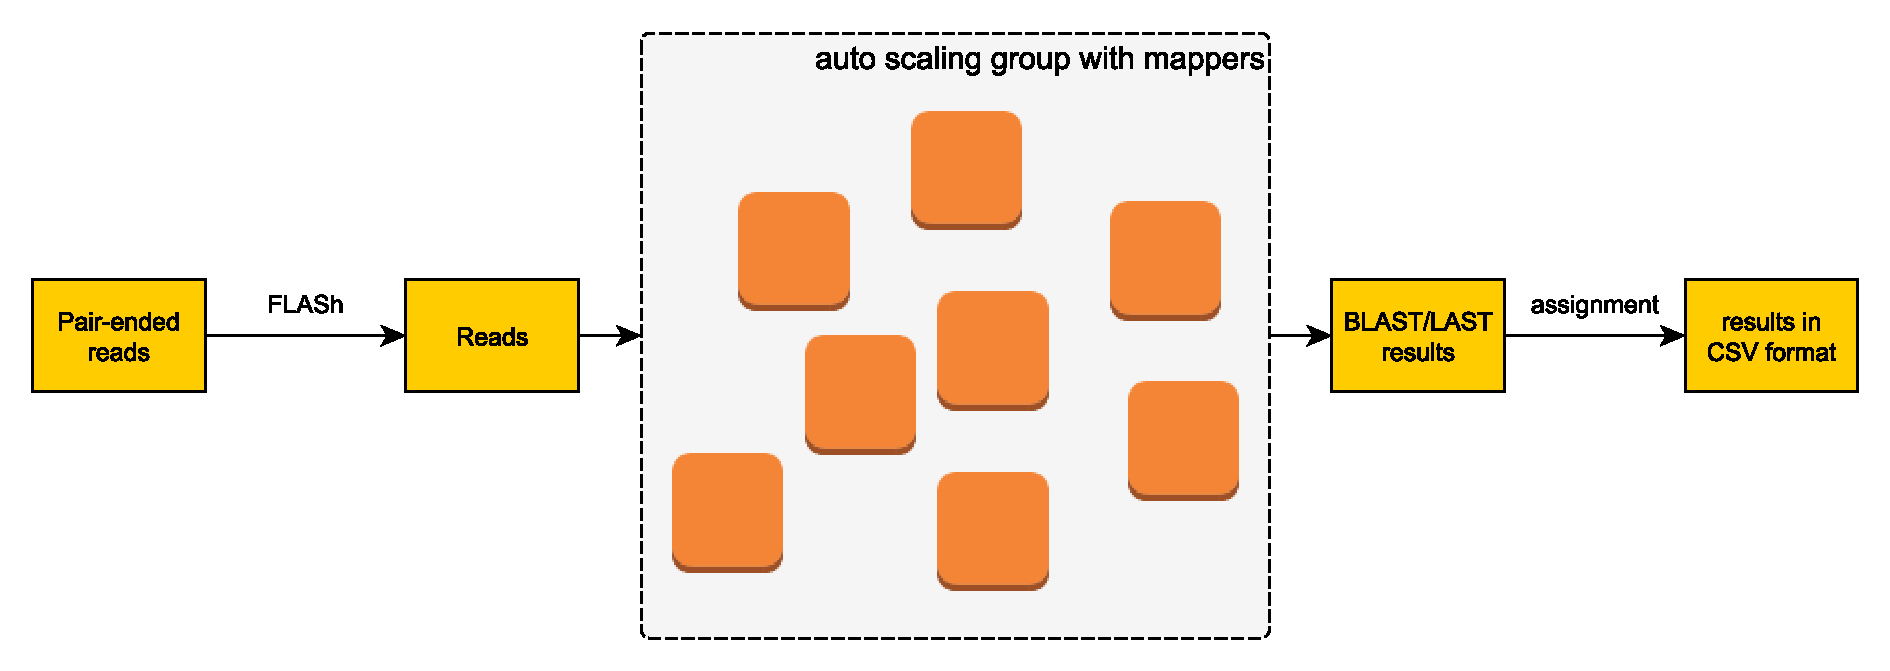
\includegraphics[width=\textwidth]{pipeline_dist.pdf}
\end{frame}



\begin{frame}
\frametitle{Cloud solution. Data management}
Besides computations Metapasta uses AWS for all data management:
\begin{itemize}
  \item input data -- samples are stored in S3
  \item output assignment tables and trees in PDF
  \item Metapasta can upload all reads (with assignment) to DynamoDB table 
\end{itemize}
\end{frame}



\begin{frame}
\frametitle{Nispero}
\includegraphics[width=0.7\textwidth]{nispero.png}
\begin{itemize}
  \item Scala library for building distributed systems
  \item Dedicated to provide maximal level of scalability and availability
\end{itemize}
\end{frame}

\begin{frame}
\frametitle{Nispero}

\begin{itemize}
  \item Amazon auto scaling groups
  \item SQS queues
\end{itemize}
\end{frame}

\begin{frame}
\frametitle{Monoids}
$$ Reads \otimes Reads \xrightarrow{merge} Reads \xrightarrow{BLAST} AssignTable \otimes Reads $$

\end{frame}


\begin{frame}
\frametitle{Bio4j}

\begin{columns}[T]
		\begin{column}{.5\textwidth}
			\includegraphics[width=\textwidth]{bio4j.png}
		\end{column}
		\begin{column}{.5\textwidth}
			NCBI taxonomy
		\end{column}
	\end{columns}
\end{frame}







\begin{frame}
\frametitle{INTERCROSSING}
This project is funded in part by the ITN FP7 project INTERCROSSING (Grant 289974).

\begin{columns}[T]
		\begin{column}{.5\textwidth}
			\hspace{.25\textwidth}\includegraphics[width=.5\textwidth]{intercrossing.png}
		\end{column}
		\begin{column}{.5\textwidth}
			\hspace{.25\textwidth}\includegraphics[width=.5\textwidth]{mc.jpg}
		\end{column}
	\end{columns}
\end{frame}


\begin{frame}
\Huge{\centerline{Thank you for your attention!}}
\end{frame}
\end{document}